%!TEX TS-program = Arara
% arara: pdflatex: {shell: yes}
\documentclass[helvetica,11pt,ngerman]{europecv}

\usepackage{ifthen}

\newboolean{papers}
\setboolean{papers}{false} 

\usepackage{graphicx,csquotes}
\usepackage{eso-pic}
\ecvLeftColumnWidth{5.7cm}
\ecvname{Donald Duck}
\ecvaddress{Arme-Schlucker-Weg 1, 12345 Entenhausen}
\ecvtelephone{0800-1234878}
\ecvemail{donald@duck.com}

\begin{document}

\begin{europecv}
\ecvpersonalinfo

\AddToShipoutPicture*{\put(440,650){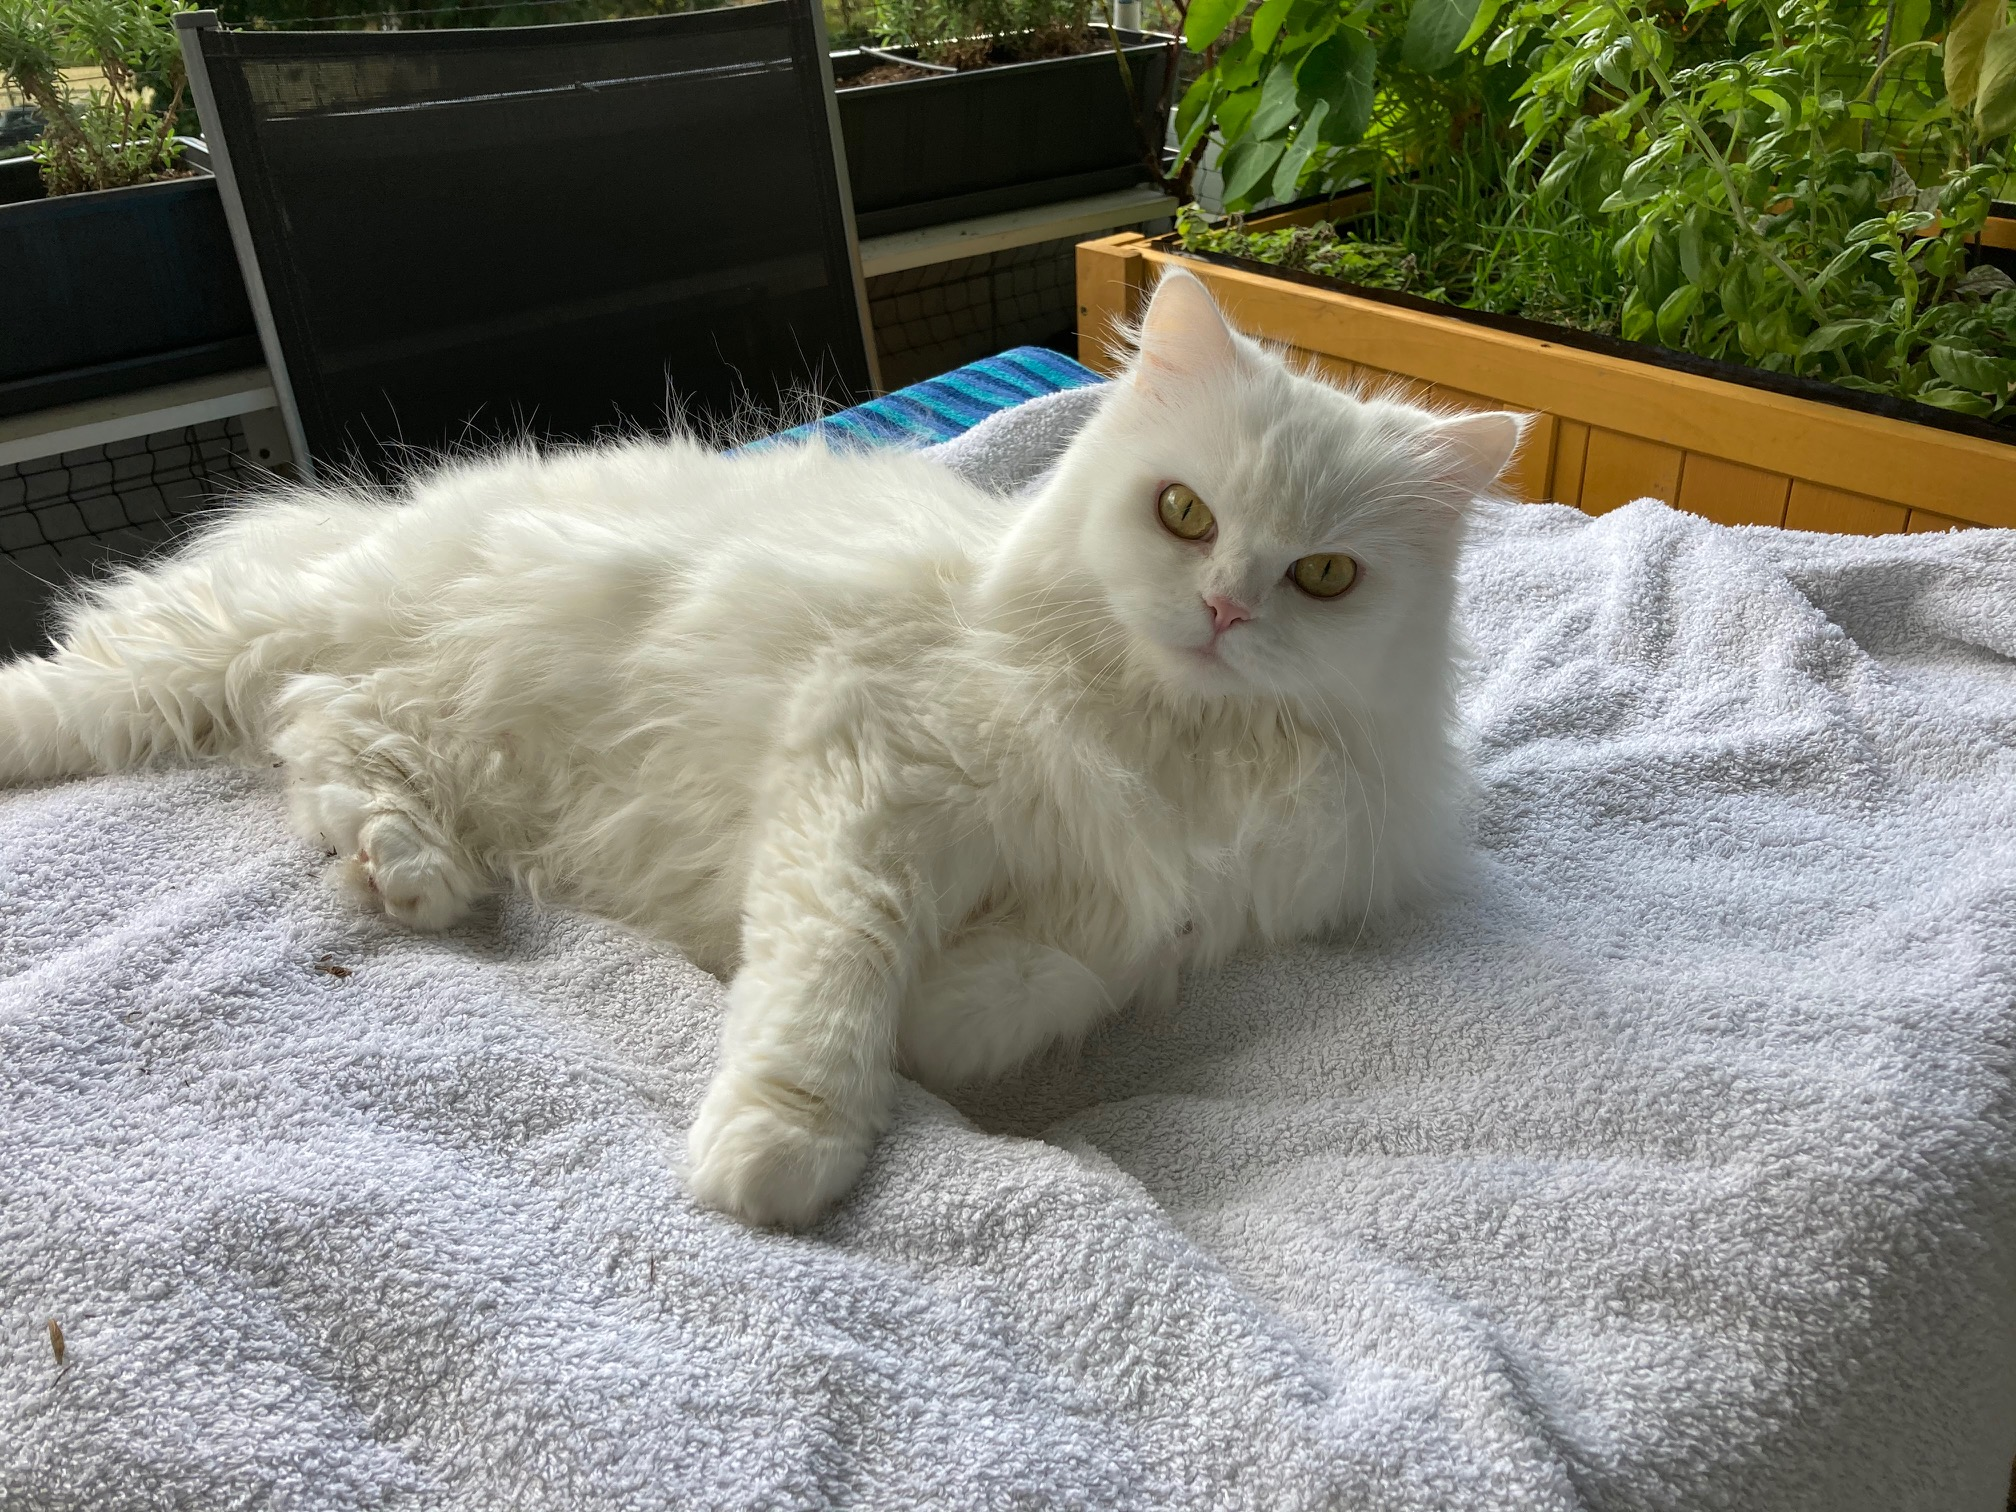
\includegraphics[height=3.5cm]{Bilder/Katze1}}}

\ecvsection{Arbeitserfahrung}

\ecvitem{2015--heute}{Handlanger bei Onkel Dagobert}

\ecvitem{}{}
\ecvitem*{Dates (from--to)}{\textbf{10/2015--12/2019}}
\ecvitem*{Name of employer}{IKB Deutsche Duckbank}
\ecvitem*{Type of business or sector}{Banking}
\ecvitem*{Corporate Title}{Handlungsbevollmächtigter}
\ecvitem*{Main activities and responsibilities}{Business Analyst \enquote{Credit \& Treasury Operations}}

\ifthenelse{\boolean{papers}}{
\ecvsection{Wiss. Veröffentlichungen}
\ecvitem{2014}{\LaTeX\ im Firmeneinsatz}
}{}
\end{europecv}

\end{document}


